
%(BEGIN_QUESTION)
% Copyright 2014, Tony R. Kuphaldt, released under the Creative Commons Attribution License (v 1.0)
% This means you may do almost anything with this work of mine, so long as you give me proper credit

Bestem riktig regulatorvirkning ({\it direkte} eller {\it revers}) for prosessen vist i figuren. Anta at både prosess-transmitter og I/P-transduser er direktevirkende (større signal inn = større signal ut):

$$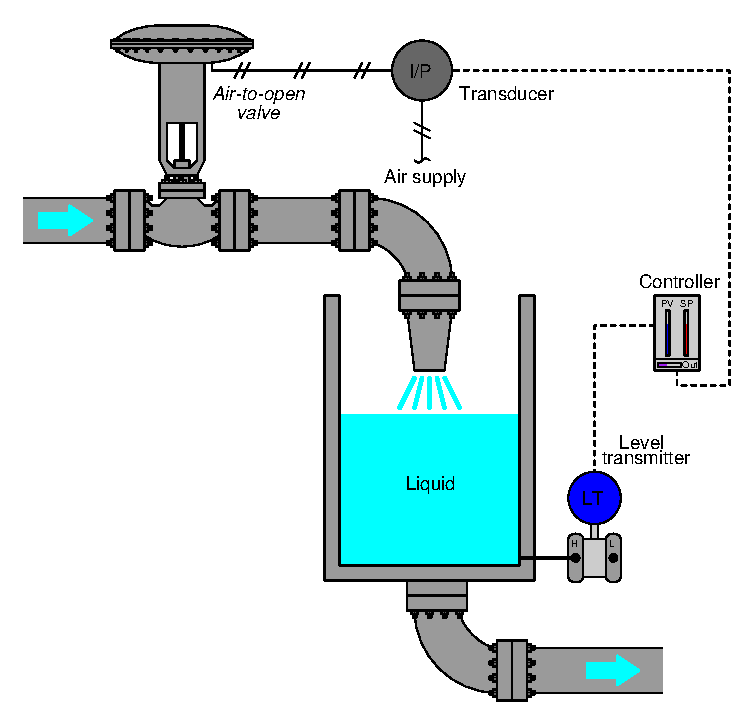
\includegraphics[width=15.5cm]{i01015x01.eps}$$

\underbar{file i01015}
%(END_QUESTION)





%(BEGIN_ANSWER)

Regulatoren bør være {\bf reversvirkende}.

%(END_ANSWER)





%(BEGIN_NOTES)

{\bf Denne oppgaven er ment kun for eksamen, ikke for arbeidsark!}.

%(END_NOTES)

